\chapter{Modell 1: YOLOX}\label{chap:yolox}
\section{Architektur}

\begin{figure}[h]
	\centering
	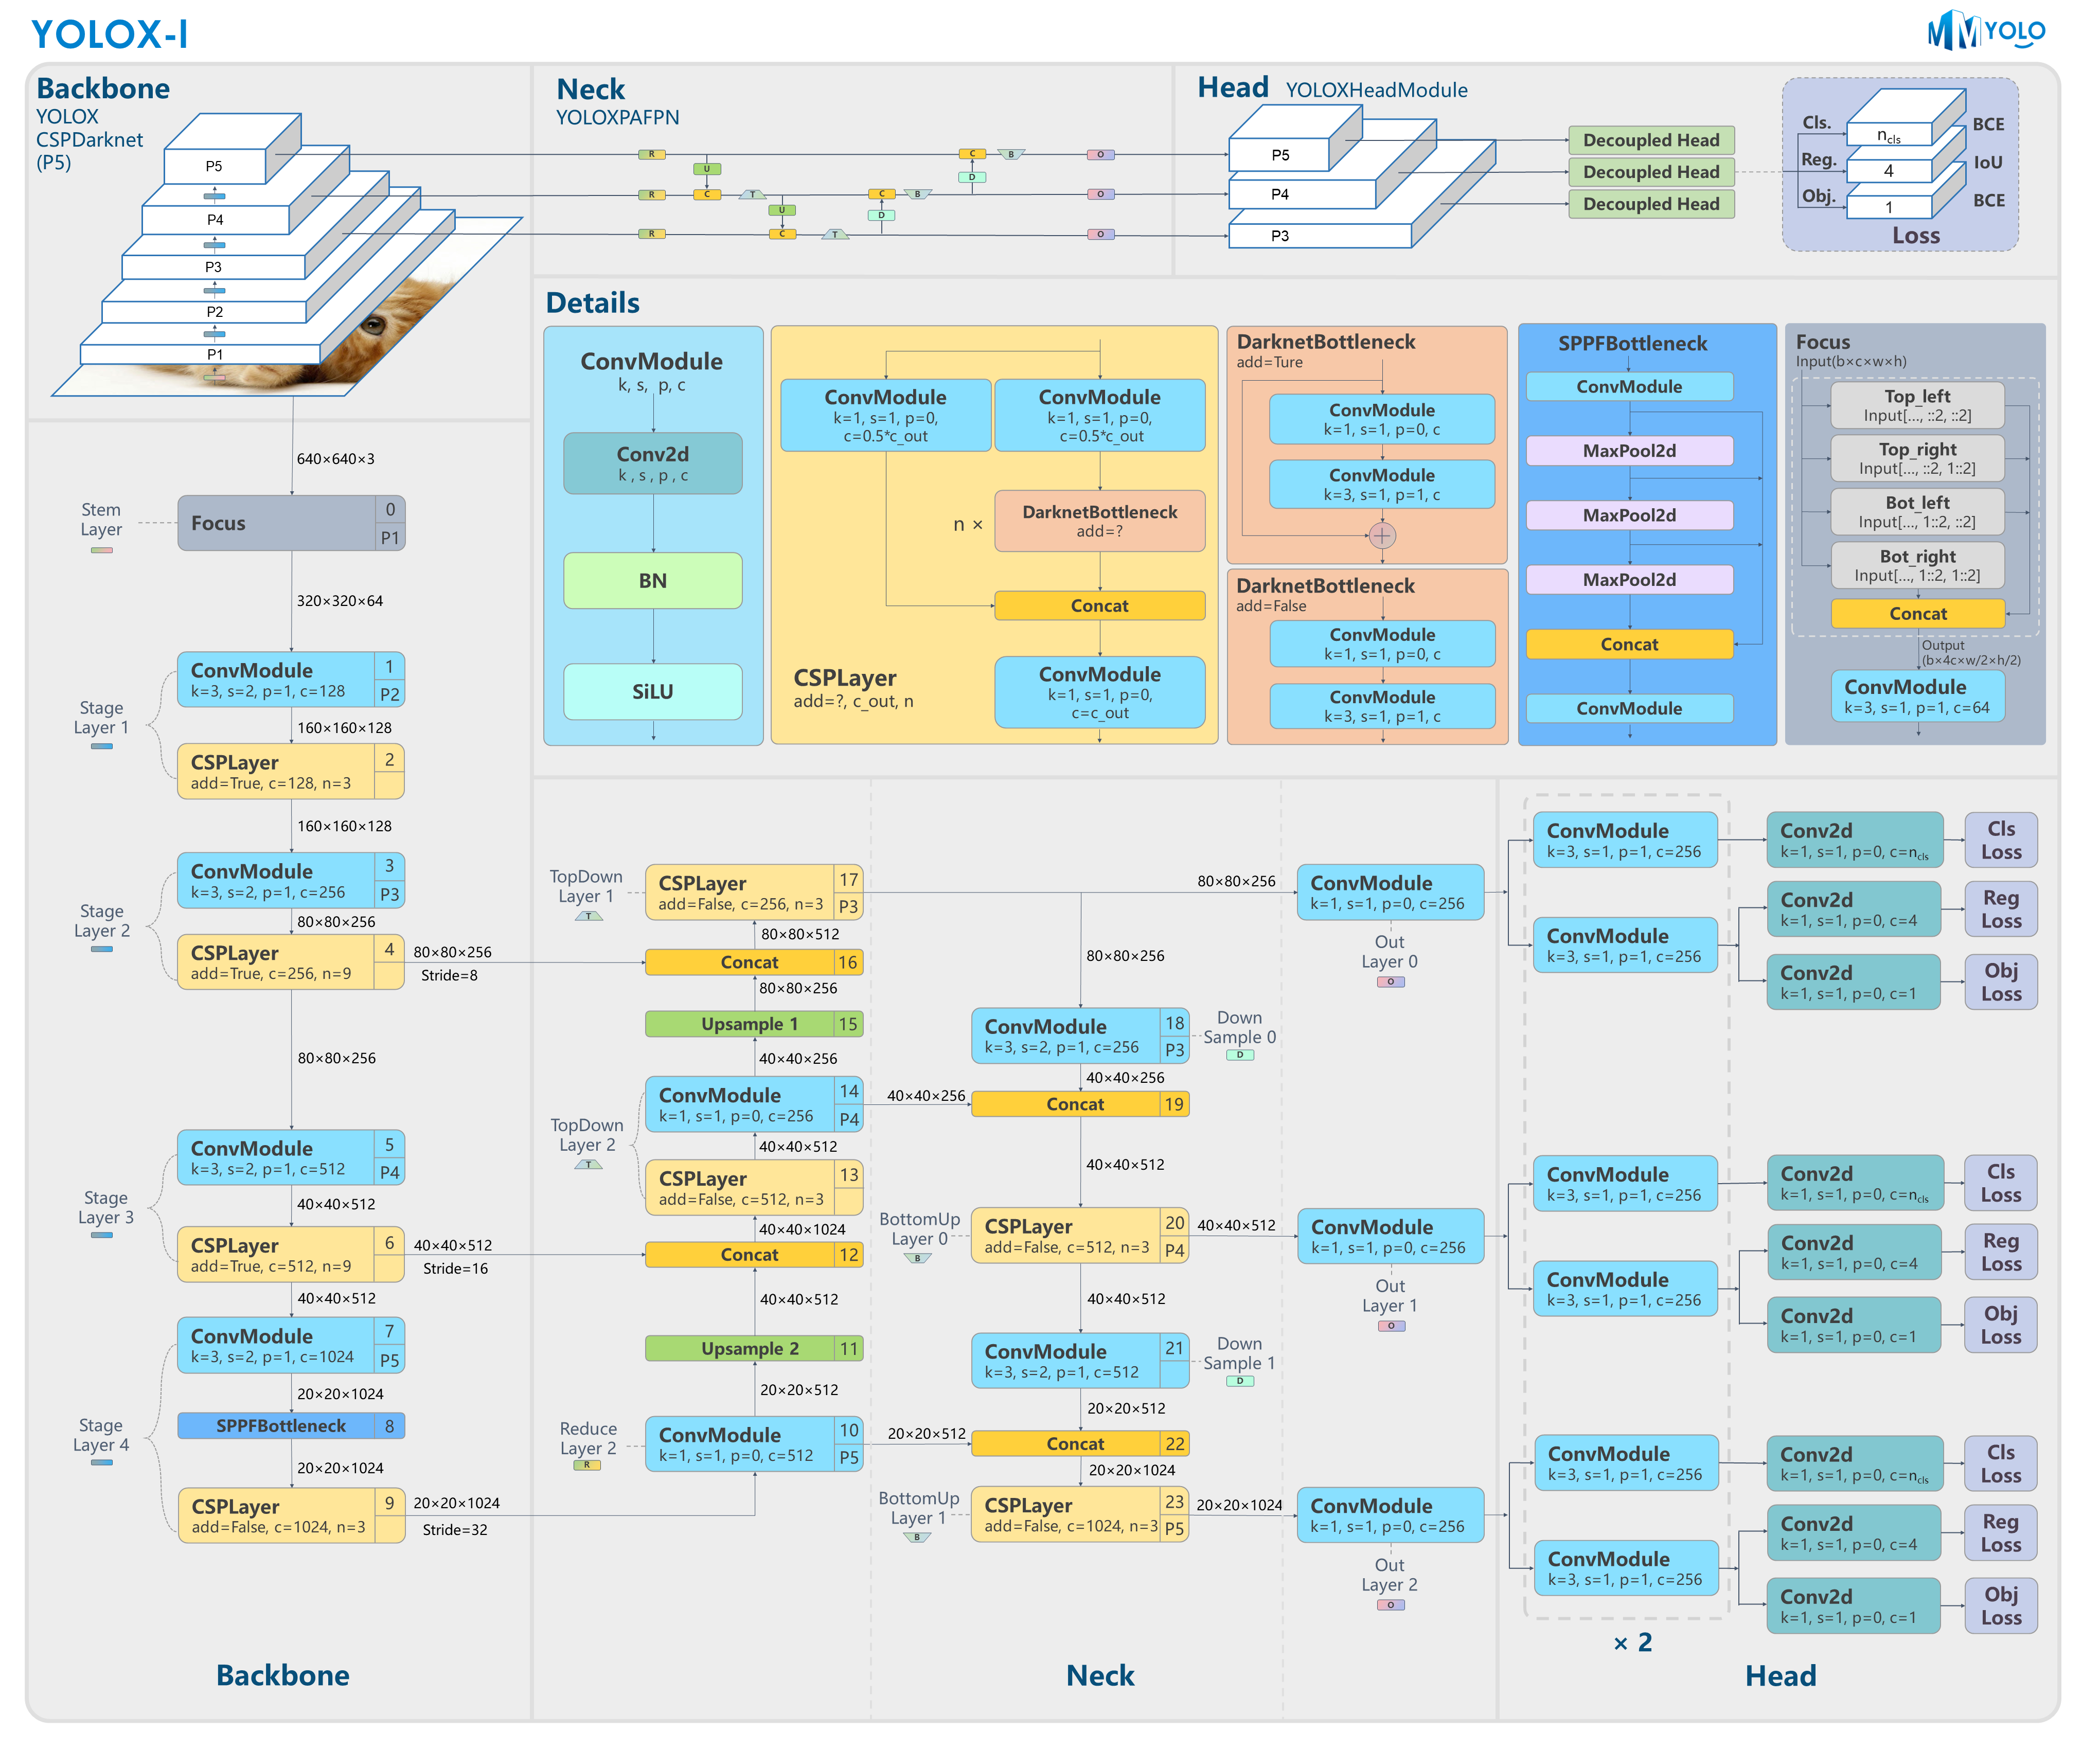
\includegraphics[width=0.8\linewidth]{yoloxArchitecture.png}
	\caption[Übersicht über die Architektur von YOLOX]{Übersicht über die Architektur von YOLOX. Quelle: \cite{yoloArchitecture, yoloxPaper, yoloxGitHubRepo}}
	\label{fig:yoloxArchitecture.png}
\end{figure}

Die YOLOX Architektur besteht aus einem Backbone-Netz, dem Neck und einem Head.

\subsection{Backbone}
YOLOX verwendet das CSPDarknet als Backbone, um Merkmale auf drei verschiedenen Maßstäben zu extrahieren. Die Ausgänge haben Dimensionen von ($H/8$x$W/8$x$256$), ($H/16$x$W/16$x$512$) und ($H/32$x$W/32$x$1024$). Diese Skalierungen ermöglichen die Erzeugung von Merkmalen für unterschiedliche Größen von Objekten. Durch die erhöhte Anzahl von Kanälen wird der Informationsverlust in den kleineren Feature-Maps ausgeglichen. Die tiefere Feature-Map (auf der Abbildung \ref{fig:yoloxArchitecture.png} unten) besitzt ein größeres Receptive Field und ein Pixel kodiert Informationen über einen größeren Bereich des ursprünglichen Bildes.

Das CSPDarknet (Cross Stage Partial) ist eine Modifizierung des ursprünglichen Darknet-Frameworks, das in YOLOv3 schon implementiert wurde. Die Anpassungen bieten Verbesserungen in Bezug auf Geschwindigkeit und Genauigkeit bei der Erkennung von Objekten in Bildern.

CSP steht für Cross Stage Partial Network. Diese Architektur besteht aus einem CSP-Block, der in verschiedenen Stufen des Netzwerks eingefügt ist. Der CSP-Block spaltet den Eingang in zwei Zweige auf, wobei ein Teil unverändert durch den Block läuft und der andere Teil durch eine Kombination aus Faltungsoperationen und Verbindungsschichten verarbeitet wird. Ziel der Kombination ist, dass das Netzwerk auf unterschiedlichen Ebenen des Netzwerks effektiver zu erfassen.

In dem Backbone wird außerdem noch am Ende der Verarbeitung ein SPP verwendet. SPP steht für Spartial Pyramid Pooling. Sie ermöglicht es Objekte unterschiedlicher Größen besser zu erkennen. Dass SPP-Modul teilt das Eingangsbild auf und reduziert die Dimensionen mithilfe von mehreren Pooling Operationen. Die unterschiedlichen Stufen werden anschließend wieder miteinander verbunden und weitergereicht. Ziel dieses Modul ist es Informationen von verschiedenen Skalierungen zu verbinden, um eine verbesserte Erkennung von Objekten zu gewährleisten. \cite{yoloxBackbone}

\subsection{Neck}
YOLOX verwendet im Neck das PAFPN (Path Aggregation Feature Pyramid Network). Dies ist eine Kombination des PAN (Path Aggregation Network) und dem FPN (Feature Pyramid Network). 

Das PAN ist verantwortlich für ds Zusammenführen von Informationen aus verschiedenen Netzwerkpfaden und die Integration dieser Informationen in einen einzigen Merkmalssatz. Es verbindet die Ausgänge des Backbone-Netzwerks auf unterschiedlichen Skalierungsebenen und passt die Dimensionen durch Upsampling aneinander an. Dadurch soll das Netzwerk ein umfassenderes Verständnis über die aus dem Backbone generierten Merkmale erhalten.

Das FPN ermöglicht eine robuste Objekterkennung in Bildern unterschiedlicher Skalierungen. Das Netzwerk erzeugt eine Hierarchie von Feature-Maps auf verschiedenen Skalierungen und verbindet sie miteinander. Dadurch sollen feine Details und auch semantische Informationen erfasst werden. FPN verwendet top-down und bottom-up-Verbindungen, um die Merkmale auf verschiedenen Ebenen des Netzwerks zu aggregieren. Die mit diesem Verfahren entstehende Merkmalspyramide wird an den Head weitergegeben. \cite{yoloxNeckPAN, yoloxNeckFPN}


\subsection{Head}
Der Head befindet sich am Ende des Netzwerks und ist für die Vorhersage der Objekte und deren Positionen in den Eingabebildern zuständig. Dort wird die Verlustfunktion berechnet. YOLOX verwendet einen Decoupled Head, der aus zwei Teilen besteht. Dieser Mechanismus ist mit YOLOX neu eingeführt worden und wird in Kapitel \ref{chap:decoupledHead} beschrieben.


\section{Methoden}
\subsection{Decoupled Head}\label{chap:decoupledHead}
Der Decoupled Head trennt die Vorhersage von Objekten und Bounding Boxes in zwei Zweige auf. Zusätzlich zum Pfad der Bounding-Box wird dort der Konfidenzwert vorhergesagt. Bei den herkömmlichen YOLO-Netzwerken wird die Vorhersage (Klasse, Bounding Box und Konfidenzwert) in einer einzigen Vorhersage gemacht. Dies kann zu Schwierigkeiten bei der Erkennung von Objekten unterschiedlicher Größe führen. 

Wie in der Abbildung \ref{fig:decoupledHead} (unten) zu sehen ist, wird im Decoupled Head die Dimension des Eingangs durch eine 1x1-Faltung reduziert und anschließend in zwei Pfade aufgeteilt. Das bedeutet, dass das Modell zuerst die Präsenz von Objekten vorhersagt und in einem parallelen Zweig die Bounding-Box-Koordinaten und den Objektscore für die erkannten Objekte berechnet. Dieser Head wird für jede der drei Neck-Feature-Maps ausgeführt. \cite{yoloxExplanationHowWorks}

Die drei Tensorausgaben von YOLOX enthalten die gleichen Informationen wie die Ausgänge des großen Tensors von YOLOv3:
\begin{itemize}
\item Cls: Die Klasse jeder Bounding Box
\item Reg: Die 4 Teile der Bounding Box
\item Obj: Wie sicher ist das Netzwerk, dass innerhalb der Bounding Box ein beliebiges Objekt ist
\end{itemize}


\begin{figure}[h]
	\centering
	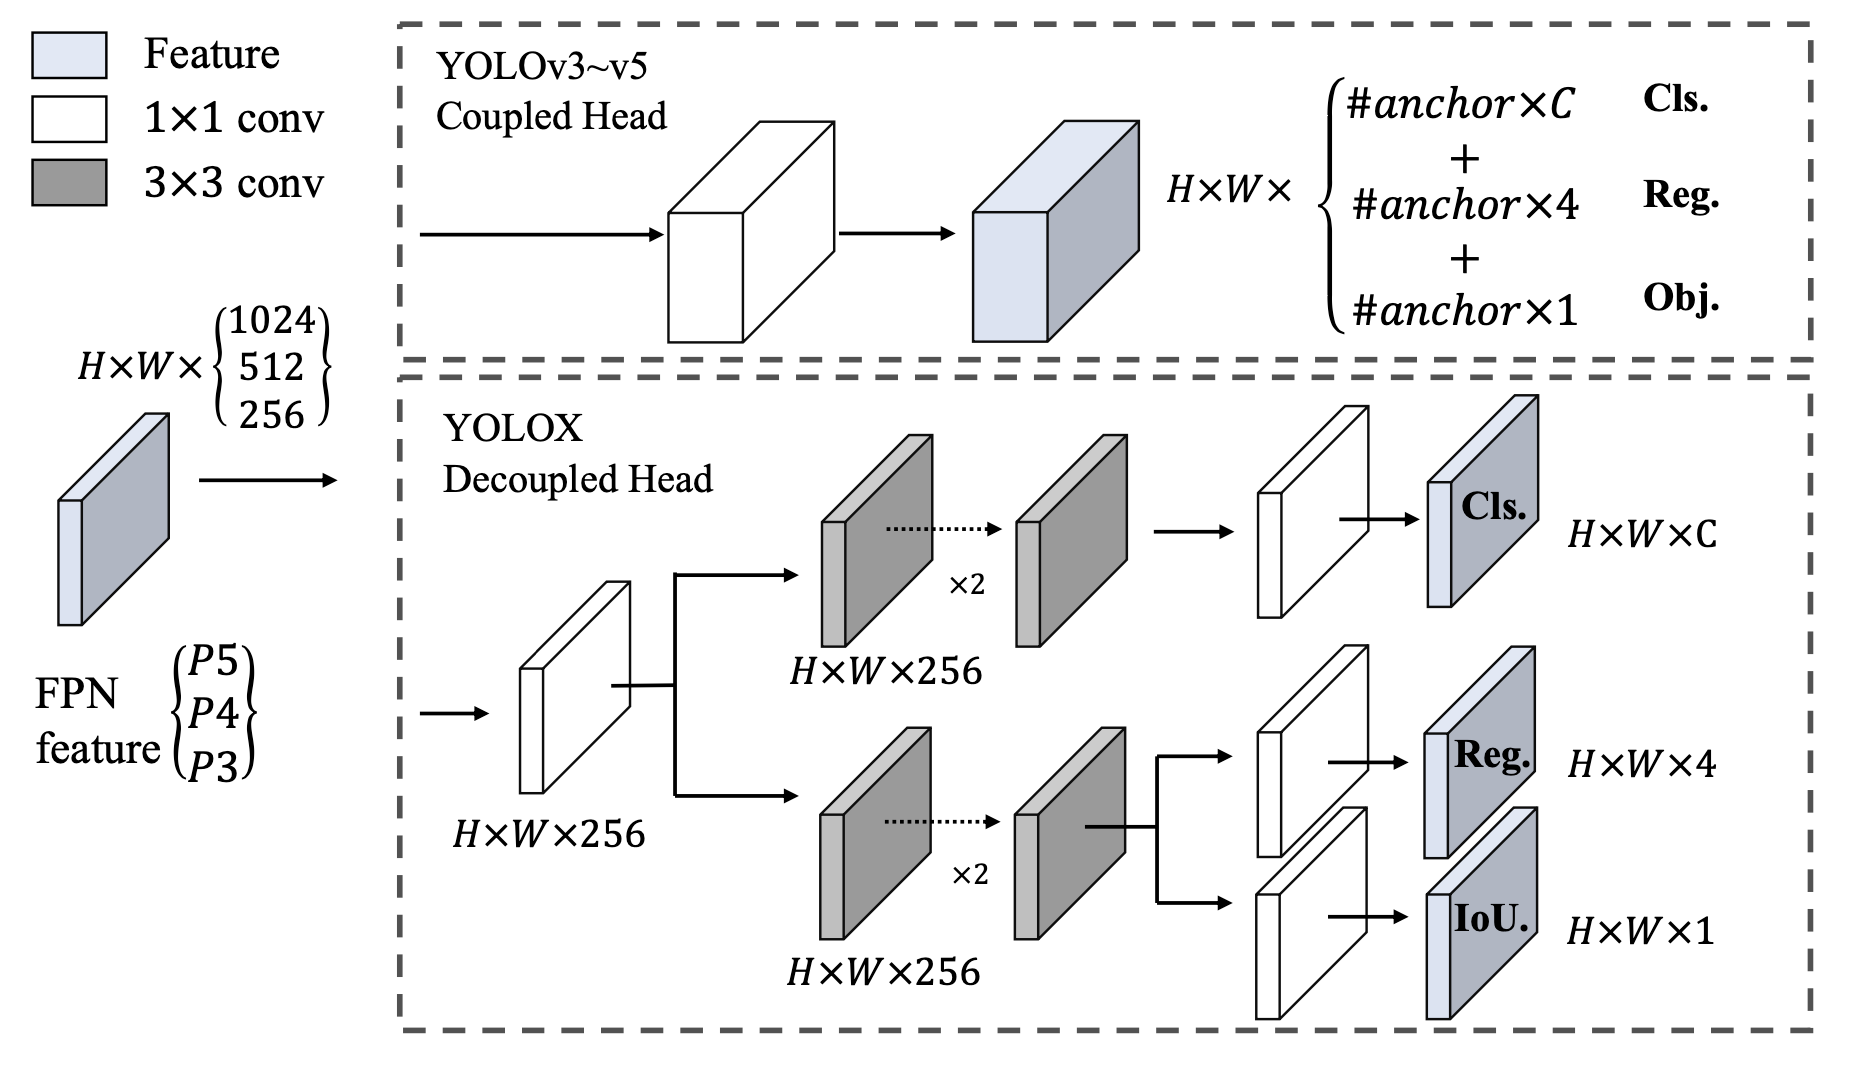
\includegraphics[width=0.55\linewidth]{decoupledHead.png}
	\caption[Illustration des Unterschieds zwischen dem Yolov3-Head und dem neuen Decoupled-Head ]{Illustration des Unterschieds zwischen dem YOLOv3-Head und dem neuen Decoupled-Head Quelle: \cite{yoloxPaper}}
	\label{fig:decoupledHead}
\end{figure}




\subsection{Anchor Free Prediction}



\subsection{SimOTA Label Assignment}


\subsection{Advanced Augmentation}


\section{Verlustfunktion}



\section{Modellauswertung}